\section{Project}
\labelsec{Project}
%===========================================================================
\subsection{Database}
Per la gestione del database si \'e scelto di utilizzare un database NoSql, nell'accezione MongoDB\cite{MongoDB}. In questa sede non si discuteranno i vantaggi, gli svantaggi o le particolarit\'a di questa tecnologia in quanto \'e stato fatto gi\'a ampiamente durante il corso. Di seguito si riportano gli schemi dei documenti che sono stati salvati, le collezioni e il significato di alcuni dei valori inseriti.

\begin{center}
\textbf{Collection Ranges}
\end{center}

In questa collezione di documenti vengono raggruppati tutti i documenti relativi ai ranges che sono da controllare. In particolare sono stati individuati due tipologie di range in base alla tipologia di sensori.

\begin{itemize}
  \item Si/No: Per quella tipologia di sensori che non forniscono effettivamente dei valori ma che notificano solamente la presenza o l'assenza di un particolare elemento come il GAS o il movimento.
  \item  Valore: validi quando un sensore effettivamente serve una misurazione di una grandezza, come ad esempio la temperatura. In questo caso \'e utile sapere se questa grandezza rimane all'interno di determinati range.
\end{itemize}
 
\begin{figure}[ht]
\centering
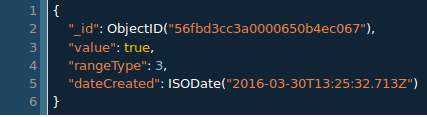
\includegraphics[width=\textwidth,natwidth=610,natheight=642]{Figures/DataStructures/RangesBoolean.png}
\caption{Documento dei Ranges Booleani}
\end{figure}


\begin{figure}[ht]
\centering
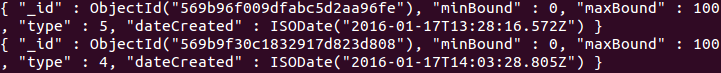
\includegraphics[width=\textwidth,natwidth=610,natheight=642]{Figures/DataStructures/RangesValues.png}
\caption{Documento dei Ranges di Valori}
\end{figure}

Si vuole far notare come sia comunque sempre presente un attributo di tipo data in modo da poter filtrare i range in base al tempo di inserimento e la presenza di un valore numerico che in questo caso rappresenta il tipo di range.

Per indicare il tipo di range si riporta il listato scala che indica tale tipologia.

\begin{figure}[ht]
\centering
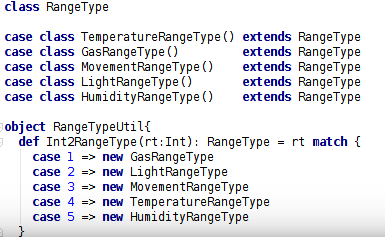
\includegraphics[scale=0.5,natwidth=610,natheight=642]{Figures/DataStructures/Ranges.png}
\caption{Valore numerico dei Ranges}
\end{figure}

\begin{center}
\textbf{Collection Data}
\end{center}

Per quanto riguarda la rappresentazione dei dati raccolti, anche in questo caso sono presenti 2 tipologie di dati:
\begin{itemize}
\item Dati Corretti: cio\'e quella tipologia di dati che rientrano all'interno del range prestabilito per la loro tipologia.
\item Dati Incorretti: quelli che invece non rientrano nella tipologia corretta e quindi vanno a violare il range attivo.
\end{itemize}

Come si pu\'o osservare il primo tipo \'e pi\'u semplice e ingloba i precedenti. Di seguito come fatto in precedenza si indica un esempio di struttura di un dato corretto e non corretto.

\begin{figure}[ht]
\centering
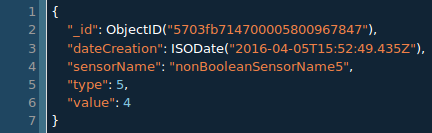
\includegraphics[scale=0.5,natwidth=610,natheight=642]{Figures/DataStructures/DataNoViolation.png}
\caption{Dato Corretto salvato in database}
\end{figure}

Come si pu\'o osservare \'e stato comunque inserito un valore per la violazione a \textit{null} in modo da poter distinguere meglio i dati violati da quelli invece corretti.

\begin{figure}[ht]
\centering
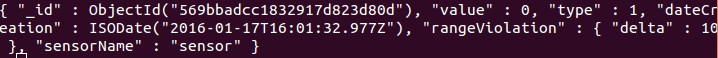
\includegraphics[scale=0.5,natwidth=610,natheight=642]{Figures/DataStructures/DataViolation.png}
\caption{Dato Non Corretto salvato in database}
\end{figure}

In questo caso appunto il valore della violazione non e' piu' nullo ma contiene un semplice campo \textit{delta} che indicher\'a la differenza rispetto al range. In particolare questo sar\'a positivo se il valore registrato supera il range attuale, negativo se invece \'e troppo basso o booleano se il tipo di sensoristica e quindi anche di range \'e booleano.

\subsection{Struttura}
\subsection{Interazione}

In questa parte si riporta la tecnologia che si \'e utilizzata per effettuare l'interazione che si \'e analizzata e indicata in fase di analisi, lo stream. In particolare si \'e notato che, il framework play\cite{PlayFramework} gi\'a gestisce attraverso delle sue strutture la possibilit\'a di operare attraverso stream di dati. Questa possibilit\'a \'e stata introdotta dal framework per gestire meglio dati parziali o casi che richiederebbero molto tempo, come ad esempio un'upload di file cospiquo. Nonostante tutto per\'o questo rientra nelle nostre necessit\'a e quindi ci avvarremo di questa astrazione per risolvere il nostro problema. Si riporta in bibliografia quindi la documentazione del framework che spiega il funzionamento di \textit{Enumerators,Iteratees e Enumeratees.} \cite{PlayStreaming}

\subsection{Comportamento}
